%%%%%%%%%%%%%%%%%%%%%%%%%%%%%%%%%%%%%%%%%%%%%

\section{Previous Work}
\label{sec:PreviousWork}
Previous work on the energy deposition of thin focused on spectra measurements from fabricated films as wells as single collision energy loss spectra.
A sequence of 10\% \iso{Li}{6}F, 5\% PPOPOPOP films in a PS matrix cast to thickness between 15 and 600 $\mu$m where fabricated and the response was measured from a gamma source as well as a neutron source.
These experiment results are shown in \ref{sec:SpectraMeasurements}.

\subsection{Spectra Measurements}
\label{sec:SpectraMeasurements}

Evidence that the secondary electrons contribute to energy loss can be seen in Figure \ref{fig:SpectraFeatures} where there is an increase in the endpoint of the spectra as films become thicker.
This increase in the spectra endpoint is indicative of the film producing more light, and as the light collection geometry remained constant the increase in the endpoint is attributed to a larger energy deposition in the 50 $\mu$m film compared to the 15 $\mu$m or 25 $\mu$m film.
%%%%%%%%%%%%%%%%%%%% Figures %%%%%%%%%%%%%%%%%%%%%%%%
\begin{figure}[h]
    \centering
    \begin{subfigure}[b]{0.45\figurewidth}
        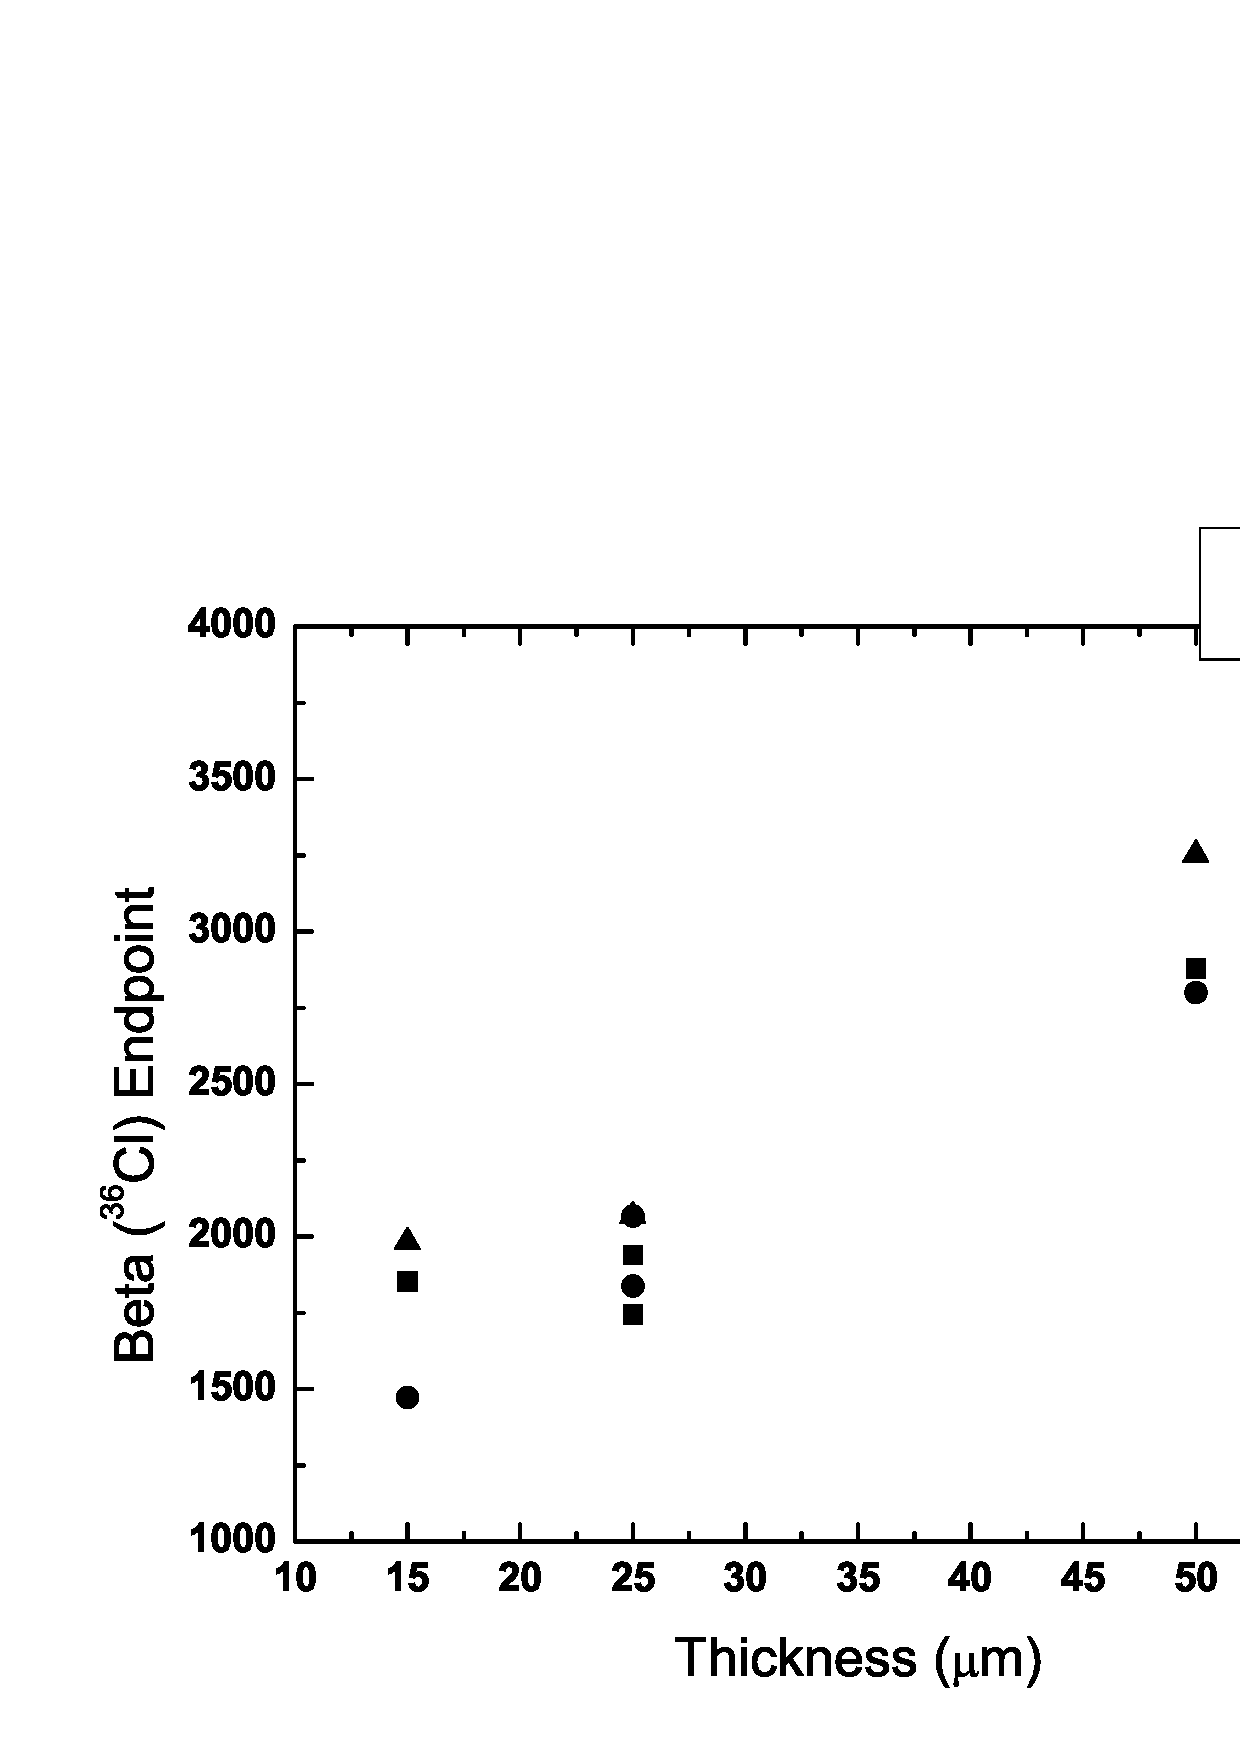
\includegraphics[width=\textwidth]{Beta}
        \caption{Beta Spectra Endpoints for a 5\% PS film}
    \end{subfigure}
    \begin{subfigure}[b]{0.45\figurewidth}
        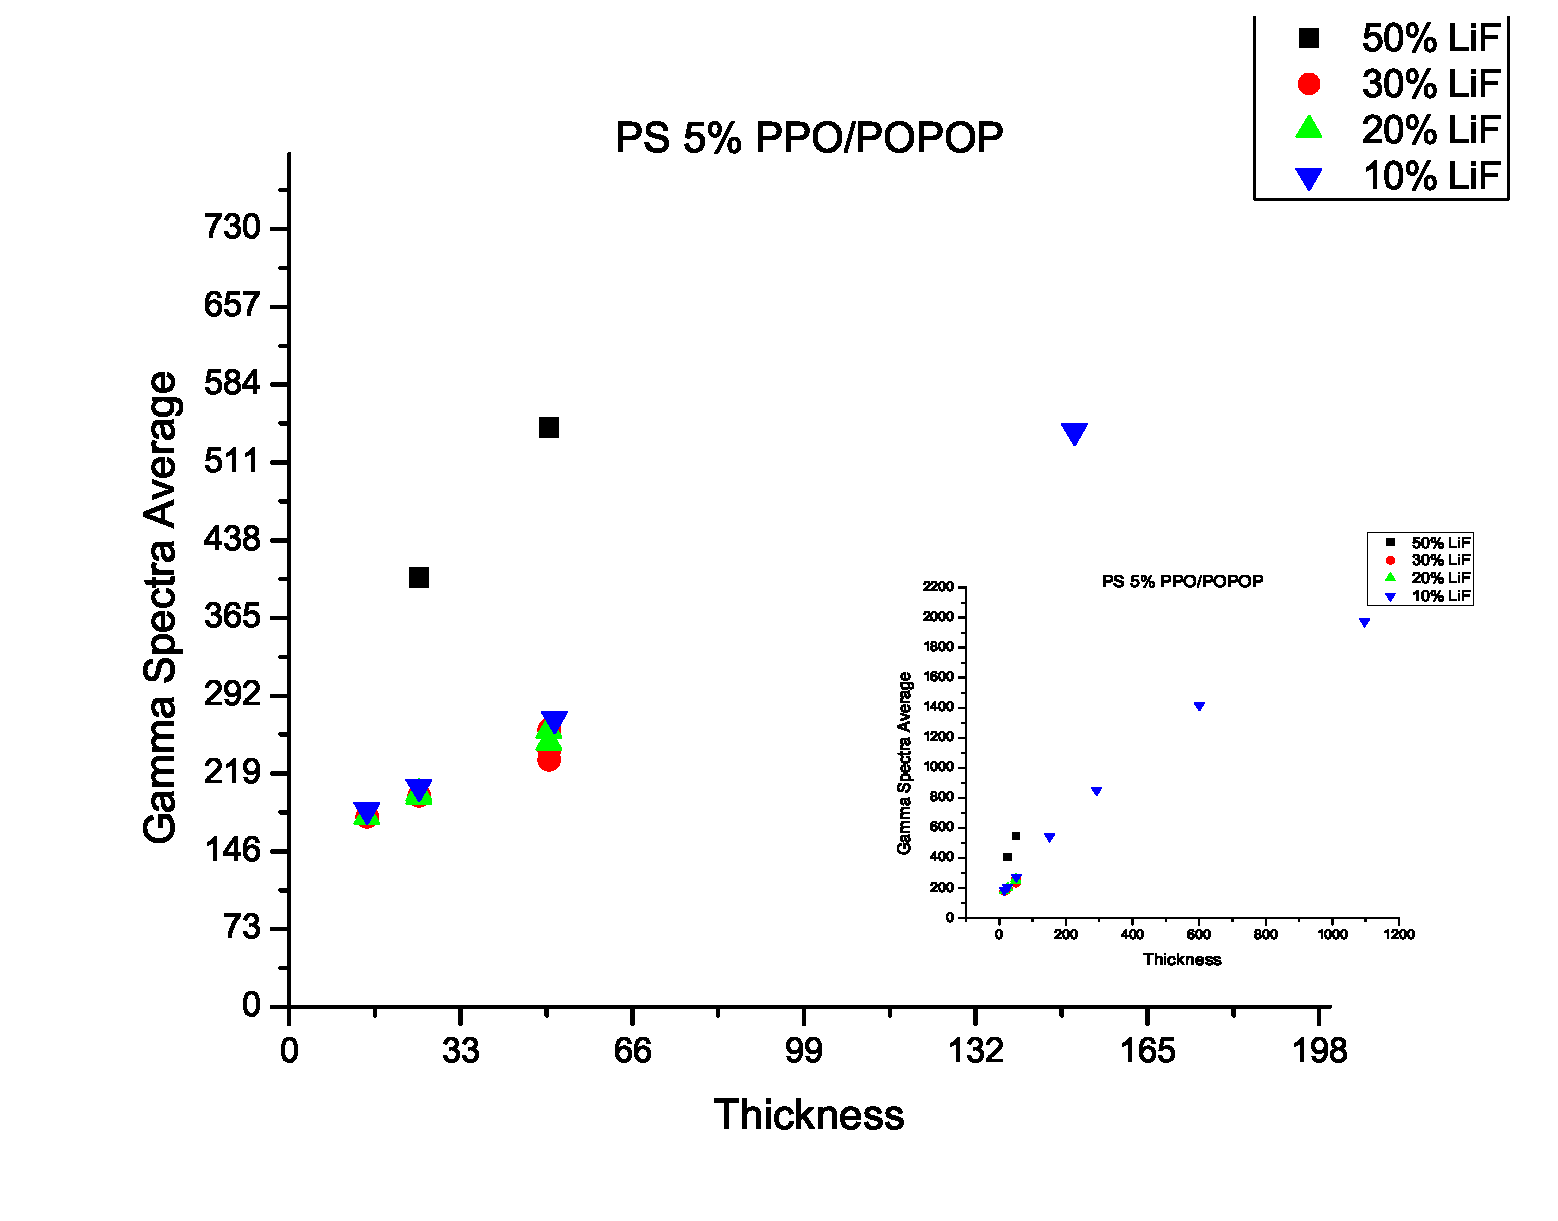
\includegraphics[width=\textwidth]{PS-5PPOPOPOP_GammaAvg}
        \caption{Gamma Spectra Averages for PS films}
    \end{subfigure}
    \caption{Spectra properties as a function of film thickness}
    \label{fig:SpectraFeatures}
\end{figure}
Figure \ref{fig:GammaIntrNeutronCounts} shows the intrinsic efficiency of these film (from spectra obtained from a \iso{Co}{60} source).
As the film thickness increases the pulse height discriminator at which an intrinsic efficiency of one in a million ($\epsilon_{int,\gamma} \le 10^{-6}$) is reached also increase.
The neutron spectra (shown in the solid lines) does not increase in light yield with increasing thickness, further providing an indication that the thickness of the films can be optimized to maximize the neutron count rates\footnote{The neutron count rate is increased with thickness by the increased mass of the detector} while minimizing the response of the detector to photons.
%%%%%%%%%%%%%%%%%%%% Figures %%%%%%%%%%%%%%%%%%%%%%%%
\begin{figure}[ht]
    \centering
    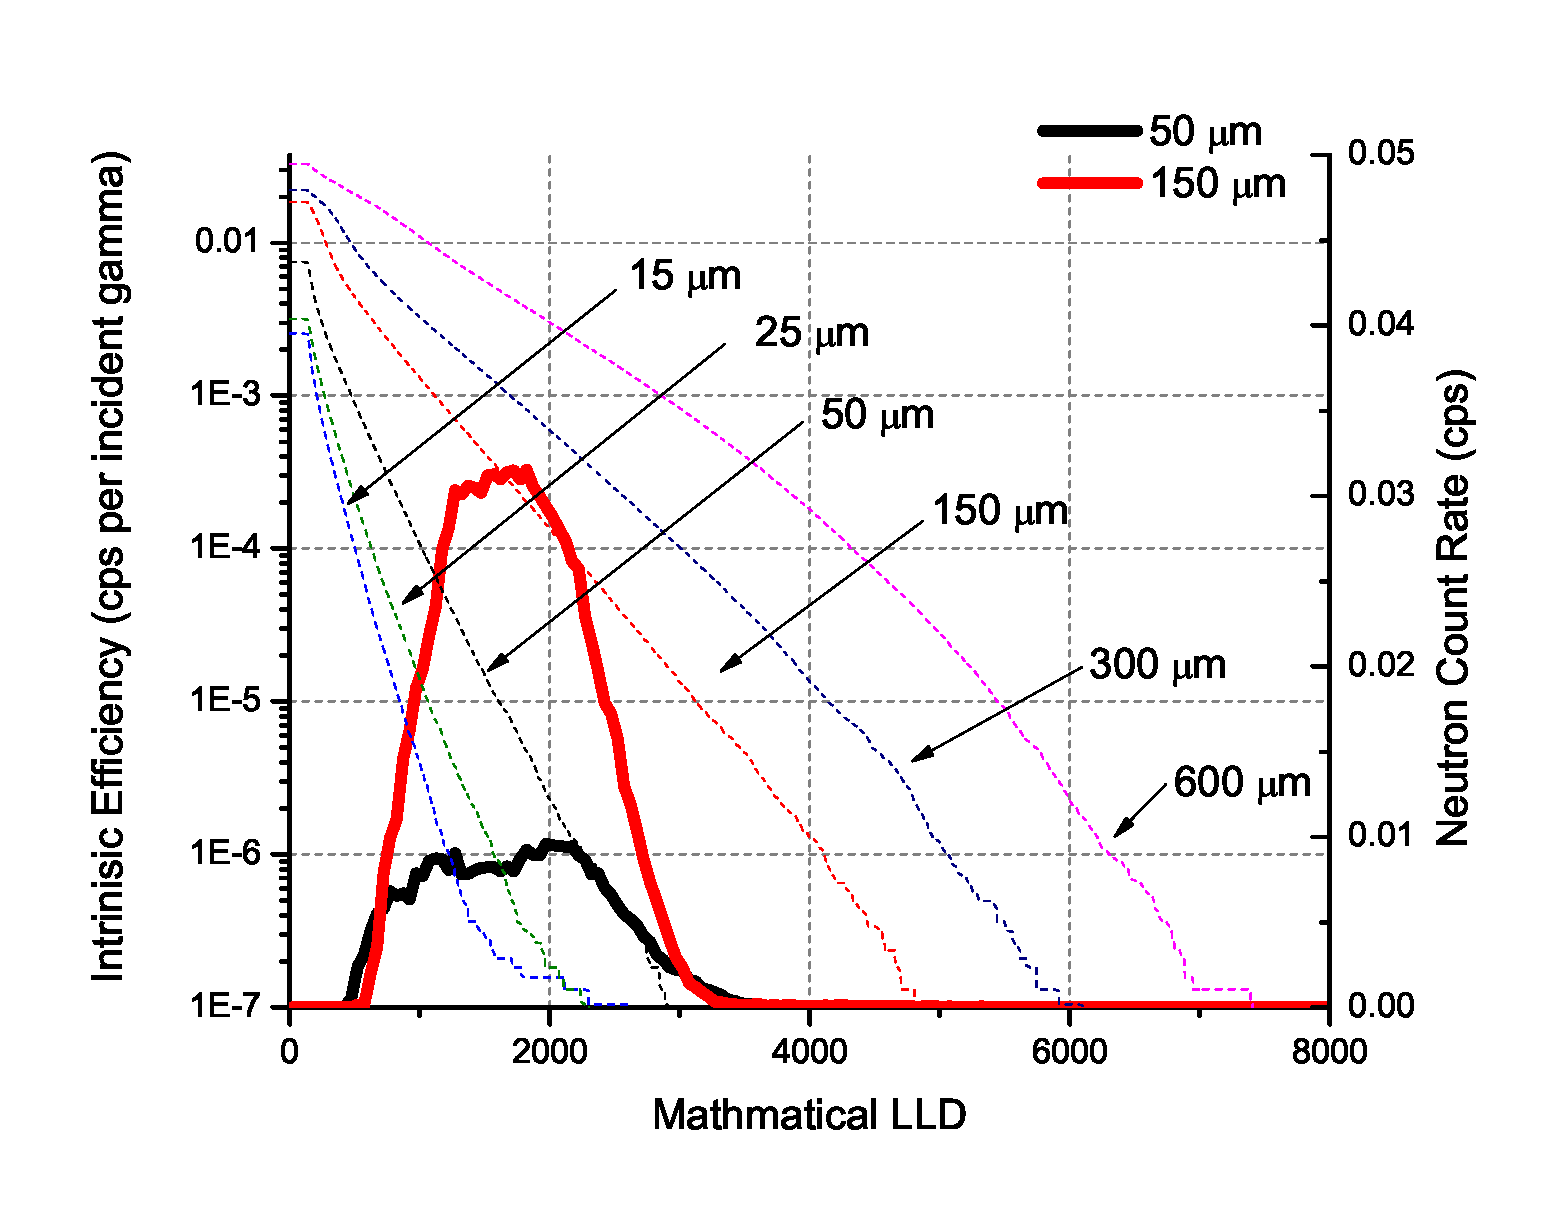
\includegraphics[width=\textwidth]{PS_IntEff_LiF20_PPO5}
    \caption{Gamma intrinsic efficiency (dashed lines) plotted against neutron counts (solid)}
    \label{fig:GammaIntrNeutronCounts}
\end{figure}

\subsection{Single Collision Energy Loss}

Single collision energy loss spectra provide the probability that that a given collision will result in an energy loss of Q.
Provided a spectra of secondary electrons from either the Compton scattered electron or the \iso{Li}{6} reaction products it is then possible to determine the average energy loss per collision.
A single collision energy loss spectra for water is shown in Figure \ref{fig:TurnerELoss}.
For low electron energies ($<$ 50 eV) it is very probable that the electron will lose a majority of its energy in a single collision.
For higher electron energies, however, the electrons tend to lose a lower fraction of there total energy. 
A Compton scattered photon, with an energy in the MeV range, will then lose far less energy per collision than an electron (in the low keV range) liberated from the passage of a neutron reaction product through the material.
%%%%%%%%%%%%%%%%%%%% Figures %%%%%%%%%%%%%%%%%%%%%%%%
\begin{figure}[ht]
    \centering
    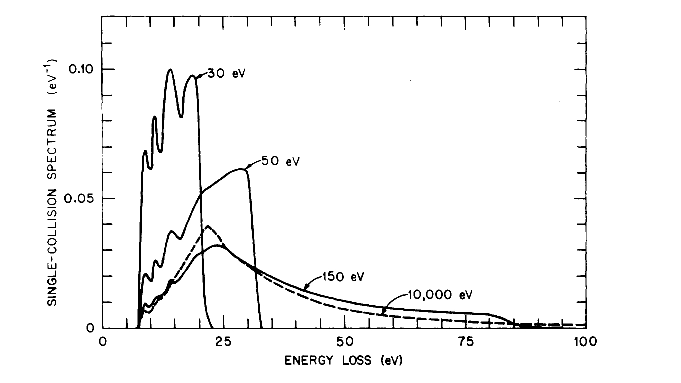
\includegraphics[width=\textwidth]{Turner_Fig2_SingleCollisionELoss}
    \caption{Single-collision energy loss spectra for electrons in water \protect\cite{turner_comparative_1982}}
    \label{fig:TurnerELoss}
\end{figure}
When the average and median energy transfer are plotted as a function of incident electron energy (Figure \ref{fig:TurnerETransfer}) the difference in the energy loss spectra becomes more apparent.
For low energies (up to an incident electron energy of 100 eV) the average and median energy transfer are roughly equal to each other, about half of the incident electron.
Past 100 eV average energy increases faster than the median energy transfer implying that while a few collisions result in large energy transfers most of the collisions do not.
It is also interesting to note that the average and median do not increase linearly with the incident energy past 100 eV (the ordinate axis is a log scale). 
In fact, the average energy transferred per collision is mostly bounded by 60 eV even for incident electron energies of \~10 keV.
This is significant because it implies that high energy electrons from photon events will deposit a small fraction of their energy in the material.
%%%%%%%%%%%%%%%%%%%% Figures %%%%%%%%%%%%%%%%%%%%%%%%
\begin{figure}[ht]
    \centering
    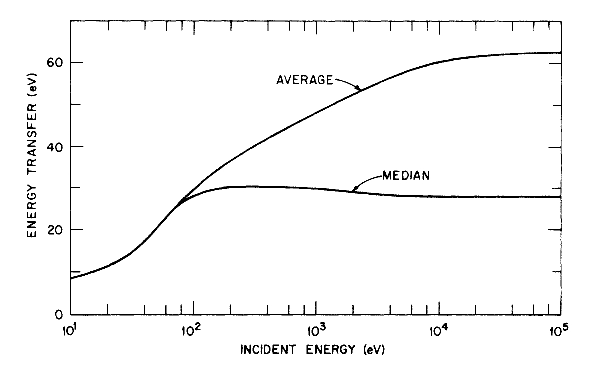
\includegraphics[width=\textwidth]{Turner_Fig3_AvgMedianETransfer}
    \caption{Average and median energy transfer in liquid water as functions of incident-electron energy \protect\cite{turner_comparative_1982}}
    \label{fig:TurnerETransfer}
\end{figure}
